%!TEX root = ../../report.tex
\chapter{Results} % (fold)
\label{cha:results}

%%%%% Introduction to the results 
% Biped designed and implemented
The bipedal locomotion platform for human-like gaits studies RuBi has been analyzed, designed and implemented.

%%%%% Statement showing where the results can be found

%%% Analysis
% physical properties analyzed
% kinematic model 
% dynamic model
% dynamic controller
During the first chapters an analysis of the problem was made giving as a result the proper conceptual definition.
The sections \ref{sec:dimensions} and \ref{sec:physical_properties} define the physical properties of the robot such what kind of materials to use or how to distribute the masses along with what are the proportions that RuBi is going to have.
It continues with the definition of each one of the joints in the section \ref{sec:joints}, where it is decided what kind of active, passive actuators and transmissions are the most appropriate for each limb.
Then, in the chapter \ref{cha:mathematical_model}, a theoretical study of the jumping case is done what is then used along with the previous sections to define a kinematic and dynamic model used to size the active and passive actuators.
This model also gives a dynamic controller used for later experiments.

%%% Electronics
% Locokit has correctly used
% The custom interface works
% ROS control correctly integrated
% The motors can be moved individually
The selection of the motors is done in the section \ref{sub:electric_actuators} and is in that electronics chapter where the LocoKit electronics are presented. 
This also includes the sensory feedback implementation in the section \ref{sub:sensory_feedback}. 
Being the result that the motors can be moved individually and concurrently which shows a valid system with the robustness and performance shown in LocoKit.
This is due to the successfully interface developed for ROS Control and LocoKit.

%%% Mechanics
% Robot designed and printed.
% Assembled
% Show photo of the robot assembled
% The mathematical model gives coherence results
% The output from the dynamic model make jump the robot in the simulation
With those constrains and the obtained from the mechanical analysis of different parts in the sections from \ref{sub:pulleys_and_belts} to \ref{sub:finite_element_method}, the CAD model is obtained.
RuBi is implemented orientated to test different spring configurations, thus a system that allows SEA, PEA or SEA+PEA is modeled and integrated into the design.
Some of the parts within the assembly have been optimized to used the modern and low-cost 3D printing FFF technologies as shown in \ref{sub:computer_aided_design}.
The robot has been successfully assembled and the output of the mathematical is coherence with the ultimate design of RuBi.
The final assembly with its bench test can be seen in the section \ref{sec:assembly}.

%%% Simulation
% Stable simulation model
% ROS control works 
% Jumps in the simulation (show picture)
% Contact sensors working too
On the simulation side, a robust and stable simulation environment has been developed.
The model is the final representation of the robot with the data obtained from the CAD program.
This assures real-like behaviors and closes the gap between the simulation and the real robot.
The simulator used, Gazebo, offers already an interface for ROS Control which leaves a complete interoperability for the controllers developed among the simulated model and the real robot.

%%% Software
The fact of using ROS opens the door to third party software that can be later implemented in RuBi without effort.
From the addition of LIDARs to IMUs or the integration of vision system, this can be done by using existing software and getting support from the community.


%%%%% Statement presenting the most important findings
% framework completed
The framework is then complete, and among the most important findings are the simplistic but realistic system to change the passive actuators and the whole set of possibilities that it offers and the implications of make a ROS enabled platform.

%statement commenting on the results this may include:
  %summary of the results
  %re-organization of the results to show trends and tendencies
  %conclusion from the results
From simulation to real life, the RuBi platform presents a good offer for researches that can work in biped locomotion controllers by reducing the spent time in maintainability of the robot or interoperability among hardware and simulation.


\begin{table}[htbp]
\caption{Physical properties of the limbs obtained from CAD program}
\begin{center}
\begin{tabular}{c|c|c|c}
 \vspace{5mm}
\large \textbf{Limb} & \large  \textbf{Length [$m$]} & \large  \textbf{Mass [$Kg$]} & \large \textbf{Moments of inertia [$Kg \cdot m^2$]} \\

Foot & 0.095 & 0.021 & \vspace{5mm} \begin{tabular}{c|c|c}
                        2.2e-005 & -9.16e-006 & 0 \\ \hline
                        -9.16e-006 & 9.05e-006 & 0 \\ \hline
                        0 & 0 & 2.88e-005 
                        \end{tabular} \\
Lower limb & 0.115 & 0.2 & \vspace{5mm} \begin{tabular}{c|c|c}
                        0.000699 & 2.44e-005 & 0 \\ \hline
                        2.44e-005 & 1.85e-005 & -1.82e-005 \\ \hline
                        0 & -1.82e-005 & 0.000694
                        \end{tabular}\\ 

Upper limb & 0.123 & 0.2 & \vspace{5mm} \begin{tabular}{c|c|c}
                        0.00119 & 2.89e-006 & -1.36e-008 \\ \hline
                        2.89e-006 & 1.69e-005 & -1.78e-005 \\ \hline
                        -1.36e-008 & -1.78e-005 & 0.00118
                        \end{tabular}\\
Hip & 0.150 & 0.156 & \vspace{5mm} \begin{tabular}{c|c|c}
                        0.000303 & 0 & 1.44e-008 \\ \hline
                        0 & 2.78e-005 & 0 \\ \hline
                        1.44e-008 & 0 & 0.000314
                        \end{tabular}\\ 
Total & & 0.707 &
\end{tabular}
\end{center}
\label{tab:limb_physical_properties}
\end{table}


\begin{figure}[tb]
  \centering
  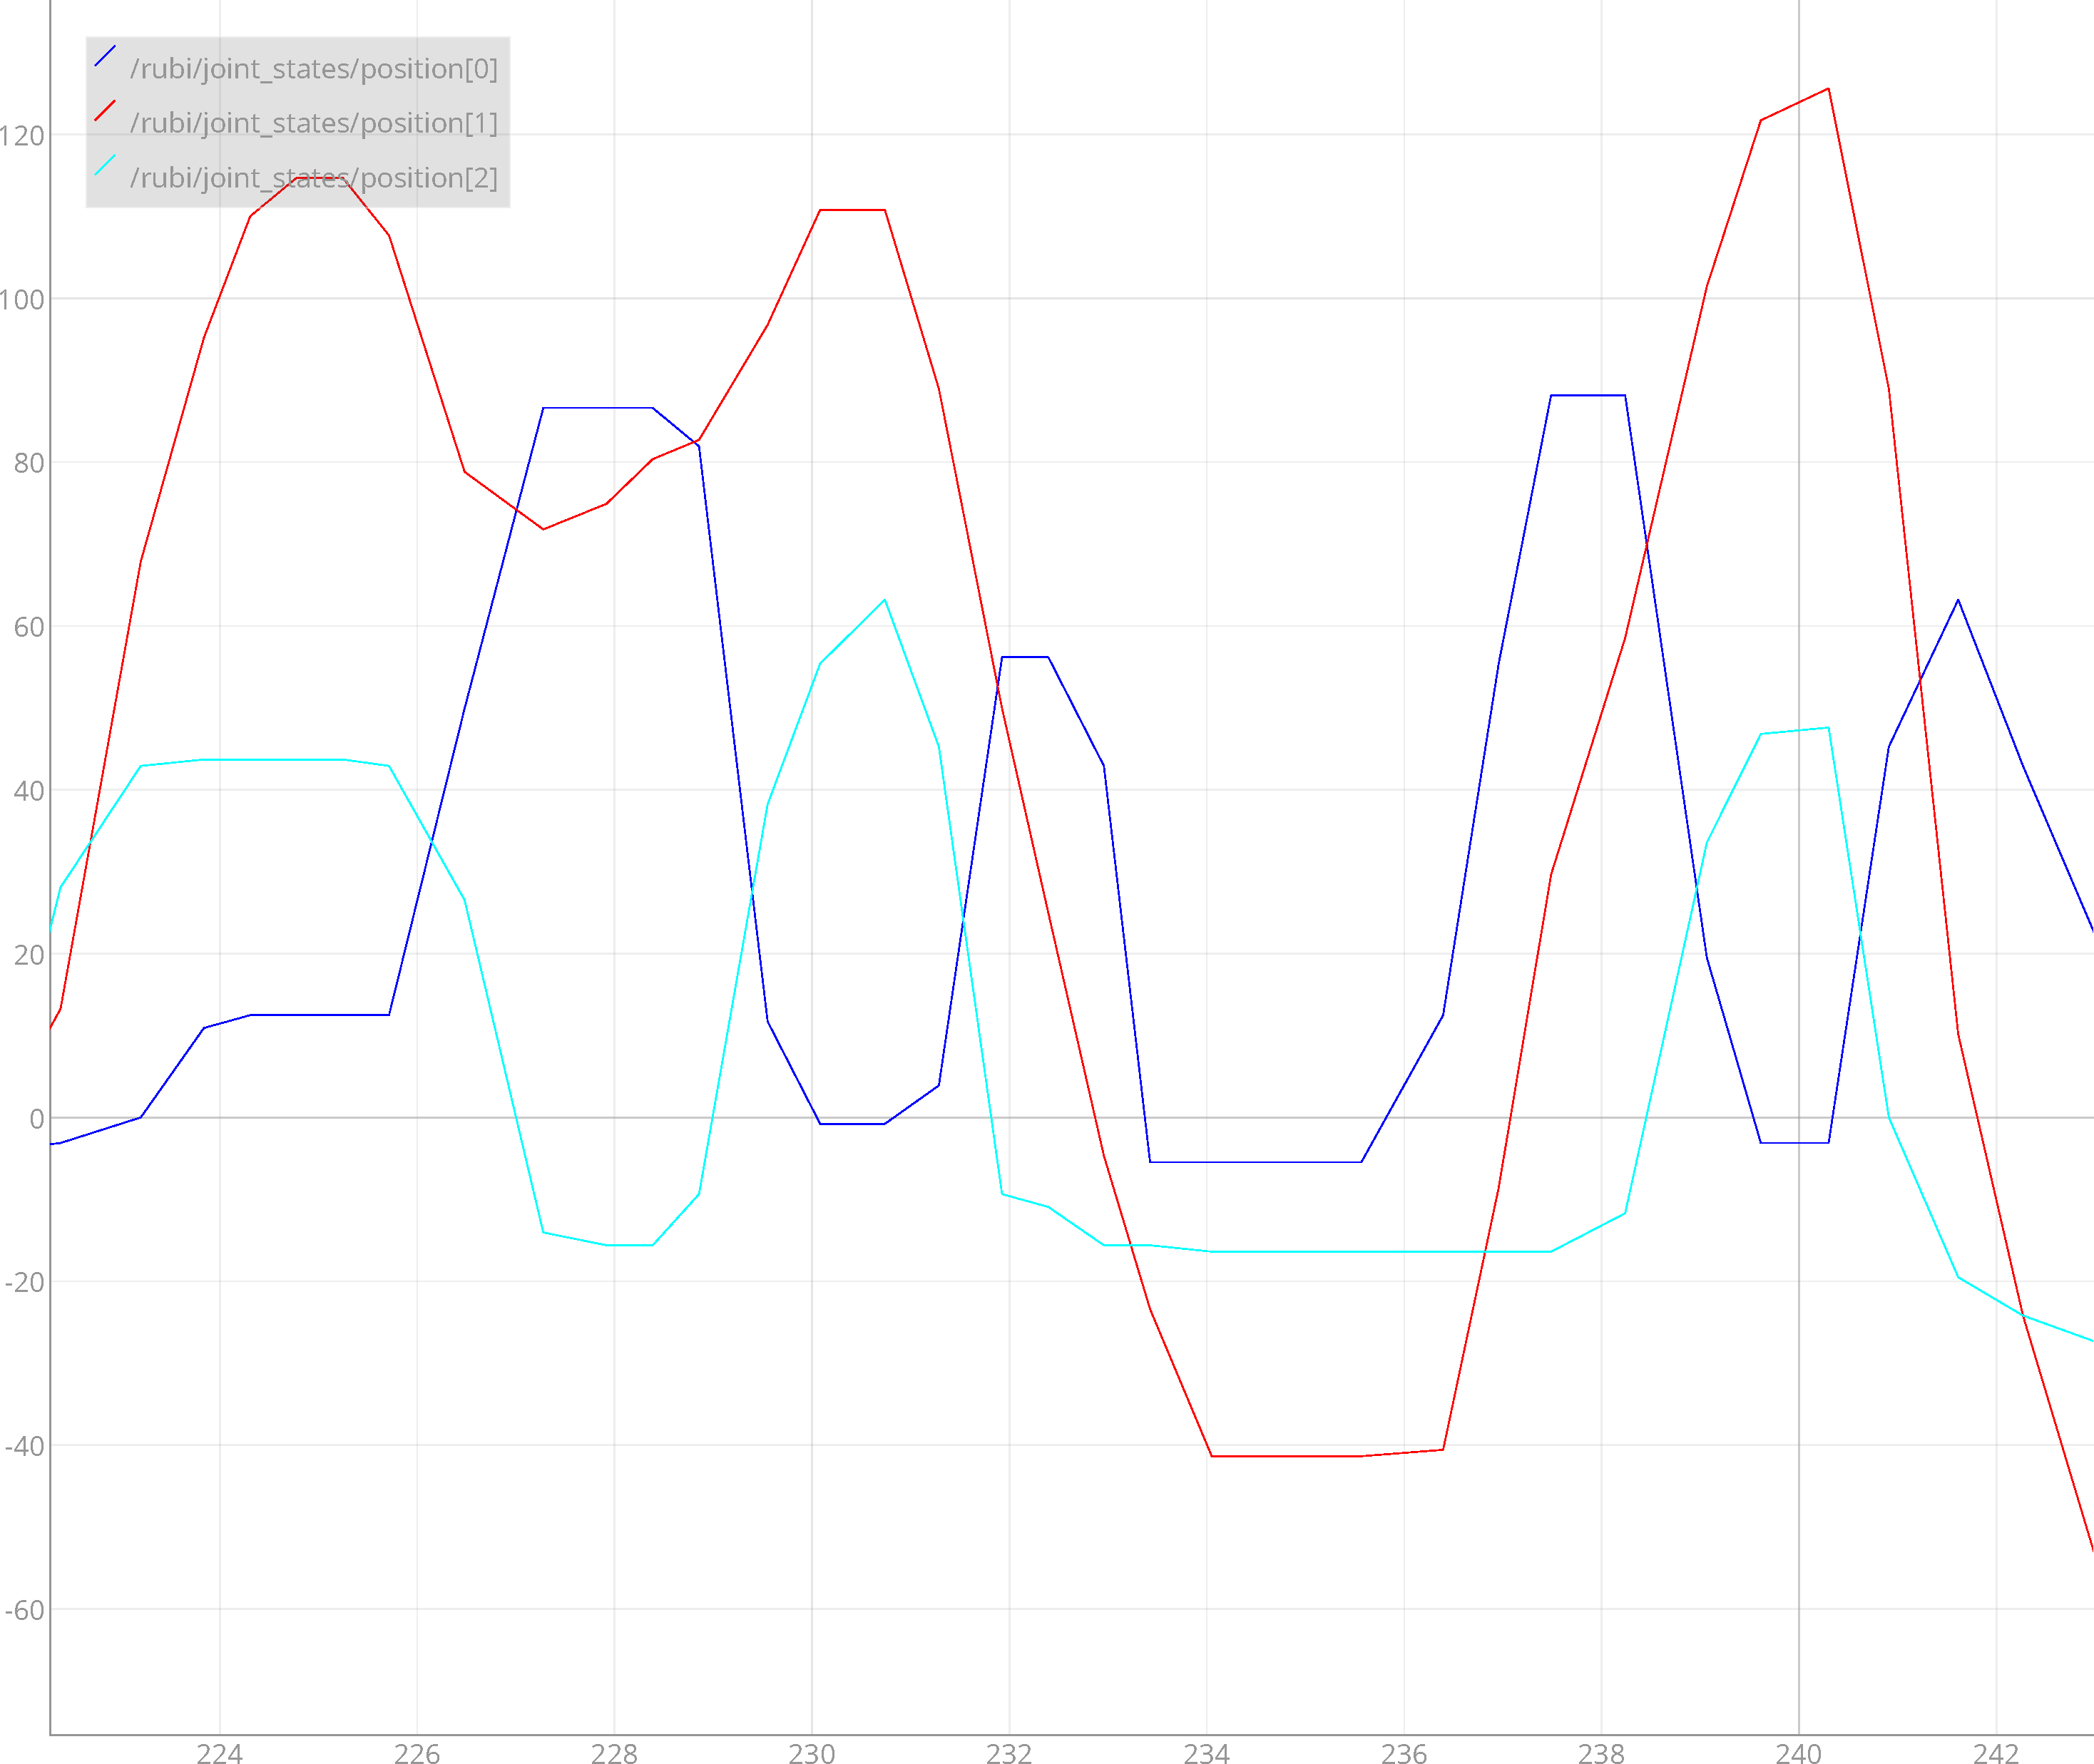
\includegraphics[width=0.75\textwidth]{figures/position_measurements.pdf}
  \caption{Measurements obtained from real robot}
  \label{fig:position_measurements}
\end{figure}
% chapter results (end)